% Very simple template for lab reports. Most common packages are already included.
\documentclass[a4paper, 11pt]{article}
\usepackage[utf8]{inputenc} % Change according your file encoding
\usepackage{graphicx}
\usepackage{url}
\usepackage{caption}
\usepackage{subcaption}
\usepackage{amsmath}
\usepackage{algorithm}
\usepackage{algpseudocode}
\usepackage{pifont}

\algdef{SE}[EVENT]{Event}{EndEvent}[1]{\textbf{upon event}\ #1\ \algorithmicdo}{\algorithmicend\ \textbf{event}}%
\algtext*{EndEvent}

\title{\textbf{Distributed Artificial Intelligence and Intelligent Agents Homework 1}}
\author{KTH Royal Institute of Technology \\ 
		School of Information and Communication Technology \\
		Student:Fanti Machmount Al Samisti (fmas@kth.se) \\
		Student:Pradeep Perris (pradeep@kth.se)}

\begin{document}
	
\maketitle

\tableofcontents

\clearpage

\section{Introduction}

\noindent The goal of this project is to implement a distributed key-value store with many freedoms given at hand like the structure, replication algorithm and factor and much more. We chose a full graph network e.g. if \textbf{n = 4} then $K_4$(in graph theory terms). 

{\centering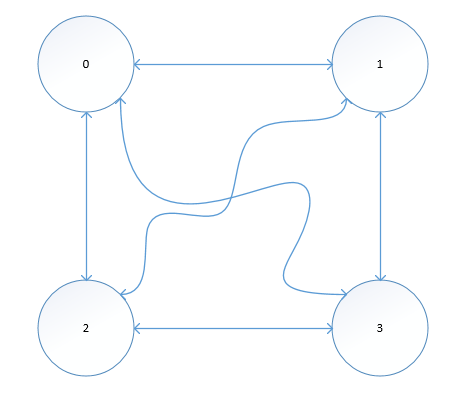
\includegraphics[scale = 0.9]{./figures/network-overview.png}\par}

\section{Enter the matrix}

\noindent Before getting deeper into the architecture of our system, an overview picture is much more effective than any description:

{\centering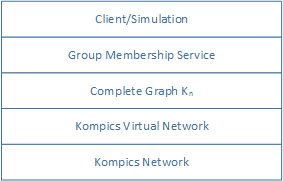
\includegraphics[scale = 0.9]{./figures/architecture.png}\par}

\noindent Having the above in mind, we can move on to the insides of our system. A \textit{Kompics} virtual network is comprised of \textit{vnodes} that share the same physical traits, namely IP address and port number, and they are distinguished by an \textit{id}. \\

\subsection{Initialization}

\noindent When then system is \textit{bootstraping}, the single \textit{NodeParent} component reads the following configuration file: 

\begin{verbatim}
network {
    node {
        host = "127.0.0.1"
        port = 34567
    }
    grid {
        num = 3 # Size of the network, has to be at least 3
    }
}
\end{verbatim}

\noindent Having done that its time to start up the nodes and create our group with the \textit{Node} components. The first node is always the initial group \textit{leader}. After him, all the subsequent nodes are \textit{slaves} and they have to send a \textit{JOIN} message to the leader to get accounted for and retrieve an updated view of the group contained in a \textit{VIEW} message. Every node is tagged with a random number whose use will be explained in the next section. \\

\noindent A possible output of the initialization phase can be the following:

\begin{verbatim}
INFO  {Node} [0]: Got JOIN message from ID: [1]
INFO  {Node} [0]: Got JOIN message from ID: [2]
INFO  {Node} [1]: Got VIEW message from ID: [0](0 1)
INFO  {Node} [1]: Got VIEW message from ID: [0](0 1 2)
INFO  {Node} [2]: Got VIEW message from ID: [0](0 1 2)
\end{verbatim}

\subsection{Key assignment} \label{keys}

\noindent We pretty much followed \textit{Chord's} key assignment algorithm and applied it to our group. With a few nodes the key assignment will not be fair but as the size increases the distribution will be normalized.

{\centering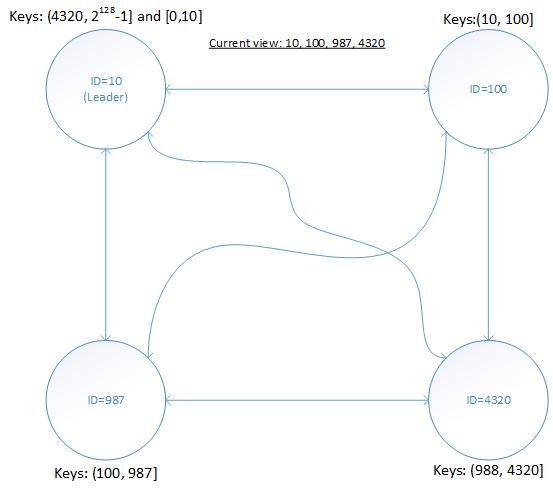
\includegraphics[scale = 0.7]{./figures/key-assignment.png}\par}

\noindent The idea here is to assign an integer range of key values to a node starting from their \textit{id} and moving  backwards until the previous nodes' \textit{id}, formally:
\begin{gather*}
range = (id_{previous}, id_{current}]
\end{gather*}

\noindent To get the keys in the desired range we apply the following formula(murmur is a hash function):
\begin{gather*}
newkey = murmur3\_128(oldkey) \mod{maxvalue}
\end{gather*}

\subsection{What's the value of XXX}

\noindent This structure wouldn't be useful if we can't send queries of \textit{GET}, \textit{PUT} and \textit{CAS}. Since this is the preliminary report we only have the \textit{GET(key)} requests for preloaded values. \\
\noindent The \textit{GET} request can be received by any node of the group. When this happens the node sends the request to the group leader, unless the leader is itself. As soon as the request arrives it gets broadcasted to the group and the ones interested in the packet respond to the client directly, aka owner node or a replica.

\subsection{Copy here, copy there, copies everywhere!}

\noindent For this system we chose to use forward replication with $\delta = 1$, as illustrated below: 

{\centering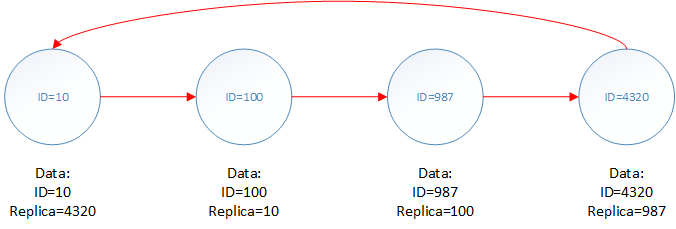
\includegraphics[scale = 0.8]{./figures/replication.png}\par}

\subsection{Who failed?}

\noindent The group is monitored by an \textit{eventually perfect failure detector}. The algorithm is shown below:

{\centering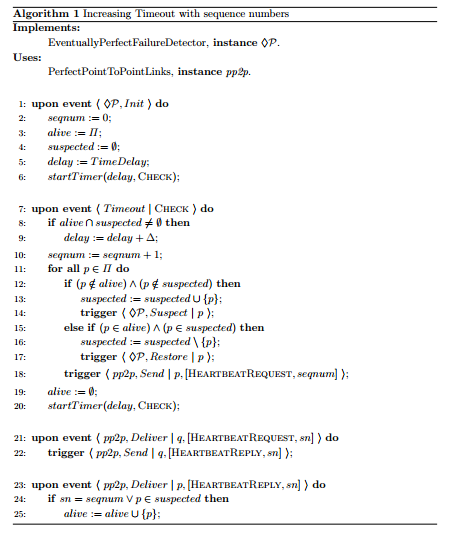
\includegraphics[scale = 0.95]{./figures/epfd-algorithm.png}\par}

\subsection{But...we should be flexible}

\noindent maybe reconfiguration insight, replication handlinig, properties(linerizable) \\

\noindent In this section we give some insight on what some of our solutions are for new, leaving and crashed nodes. \\
\noindent In the same fashion as \textit{Chord} when a \textbf{node joins} the network it should be handed over the keys that is responsible for based on its \textit{id} as described in section \ref{keys}. This is shown below:

{\centering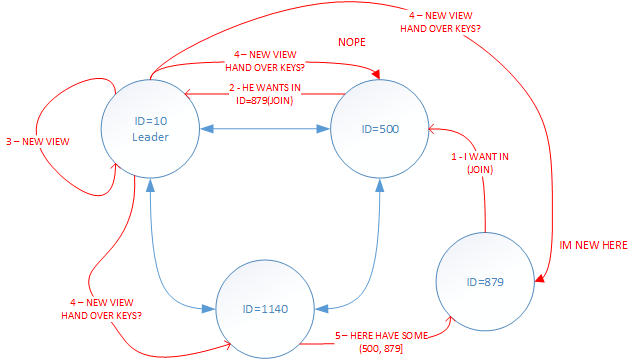
\includegraphics[scale = 0.90]{./figures/nodejoin.png}\par}

\clearpage

\noindent Based on the same logic when a \textbf{node leaves or crashes} the network should rebalance and hand keys to the proper owners in this new configuration:

{\centering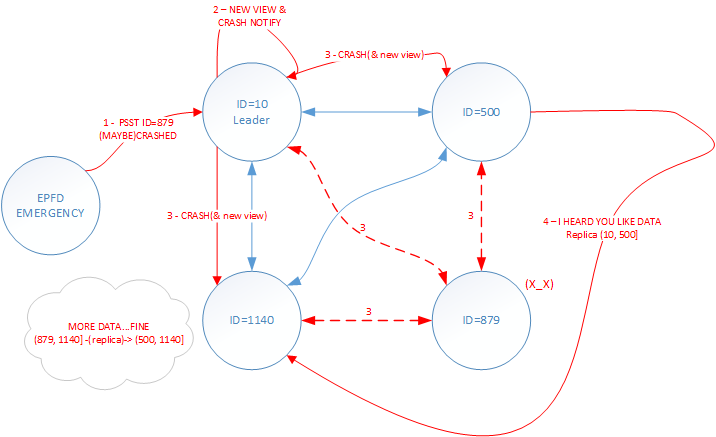
\includegraphics[scale = 0.87]{./figures/nodecrash.png}\par}

\section{References}
\begin{itemize}
	\item http://www.slideshare.net/WayneJonesJnr/chapter-16-distributed-system-structures-1314596
	\item 
	http://blog.fourthbit.com/2015/04/12/building-a-distributed-fault-tolerant-key-value-store
\end{itemize}

\end{document}
